
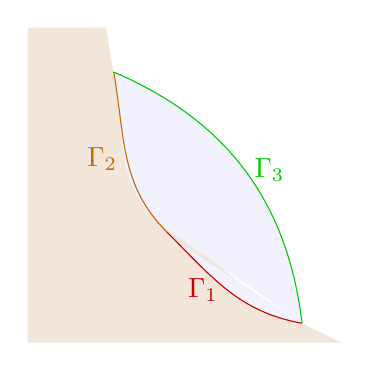
\begin{tikzpicture}

\fill[brown!20!white]
	(0,0) -- (4, 0)
	to[bend left]
		node[pos = 0.1, outer sep = 0pt] (BA) {}
		node[pos = 0.9, outer sep = 0pt] (BB) {}
		node[pos = 0.5, outer sep = 0pt, xshift = -0.15cm, yshift = -0.15cm] (BM) {}
	(1, 4) -- (0, 4) -- cycle;

\fill[blue!5!white] (BA.center)
	to[out = 170, in = -45] (BM)
	to[out = 135, in = -80] (BB.center)
	to[bend left](BA.center);

\draw[red!80!black] (BA.center)	to[out = 170, in = -45] node[midway, left] {$\Gamma_1$} (BM.center);

\draw[orange!80!black] (BM.center) to[out = 135, in = -80] node[midway, left] {$\Gamma_2$} (BB.center);

\draw[green!80!black] (BB.center) to[bend left] node[midway, right] {$\Gamma_3$} (BA.center);

\end{tikzpicture}
